% Document Header
\documentclass[tikz,border=12pt,12pt]{standalone}
\hyphenpenalty=10000
\usepackage{fontspec}
\graphicspath{{../icons/}}

\definecolor{nightblue}{HTML}{002846}
\definecolor{gray2}{HTML}{A2AAAD}
\definecolor{gray3}{HTML}{425563}

% Style for transaction flows with splitted boxes
\tikzset{
fontscale/.style={font=11pt},
solidarrow/.style={line width=2pt, gray3, ->, >=stealth},
dashedarrow/.style={line width=2pt, gray3, ->, >=stealth, dashed},
outcome/.style={rectangle,fill=nightblue,draw=nightblue,rounded corners,text=gray3,ultra thick,text width=6cm,align=center,node distance=9cm},
split/.style={
       rectangle split,
       rectangle split parts=2,
       rectangle split part fill={nightblue,white},
       rounded corners,
       draw=nightblue, ultra thick,
       minimum height=2cm,
       text width=6cm,
        text height=1.8cm, text depth=1.8cm,
       text=gray3,
       inner sep=5pt,
       text centered,
       node distance=9cm
       },
split3/.style={
       rectangle split,
       rectangle split parts=3,
       rectangle split part fill={nightblue,white,white},
       rounded corners,
       draw=nightblue, ultra thick,
       minimum height=2cm,
       text width=6cm,
        text height=1.1cm, text depth=1.1cm,
       text=gray3,
       inner sep=5pt,
       text centered,
       node distance=9cm
       },
split4/.style={
       rectangle split,
       rectangle split parts=4,
       rectangle split part fill={nightblue,white,white},
       rounded corners,
       draw=nightblue, ultra thick,
       minimum height=2cm,
       text width=6cm,
       text=gray3,
       inner sep=5pt,
       text centered,
       node distance=9cm
       }
}

% Font
%% ItalicFont=DINWebPro-Ita.otf,
%% BoldItalicFont=texgyreheros-bolditalic.otf]
\setmainfont[
  Path=../fonts/,
  BoldFont=DINWebPro-Bold.ttf,
  ItalicFont=DINWebPro-Ita.ttf
]{DINWebPro.ttf}
\newcommand\wdtocplacement{auto}
\newcommand\wdattributeundefined{drop-line}
\newcommand\wdattributemissing{skip}
\newcommand\wdtoctitle{Table of Contents}
\newcommand\wduntitledlabel{Untitled}
\newcommand\wdversionlabel{Version}
\newcommand\wdlastupdatelabel{Last updated}
\newcommand\wdasciidoctorversion{2.0.10}
\newcommand\wdsafemodename{unsafe}
\newcommand\wdsafemodelevel{0}
\newcommand\wdmaxincludedepth{64}
\newcommand\wdhtmlsyntax{html}
\newcommand\wdbackend{html5}
\newcommand\wdoutfilesuffix{.html}
\newcommand\wdfiletype{html}
\newcommand\wdbasebackend{html}
\newcommand\wdstylesdir{.}
\newcommand\wdiconsdir{./images/icons}
\newcommand\wdlocaldate{2020-02-27}
\newcommand\wdlocalyear{2020}
\newcommand\wdlocaltime{15:15:19 +0100}
\newcommand\wdlocaldatetime{2020-02-27 15:15:19 +0100}
\newcommand\wddomain{wirecard.com}
\newcommand\wdpaymentgatewayabbr{WPG}
\newcommand\wdpaymentpageabbr{WPP}
\newcommand\wdpaymentpageanchor{WPP}
\newcommand\wdpaymentpageabbrlowercase{wpp}
\newcommand\wdpaymentprovidernamelowercase{wirecard}
\newcommand\wdpaymentprovidername{Wirecard}
\newcommand\wdmermaidconfig{config/mermaid-default-theme.json}
\newcommand\wdpaymentredirecturlhostname{www.wirecard.com}
\newcommand\wdapiid{wpp}
\newcommand\wdcheckoutpagehtmlhostname{www.wirecard.com}
\newcommand\wdpaymentpagefunctionshort{WPP}
\newcommand\wdpaymentpagefunction{WirecardPaymentPage}
\newcommand\wdpaybuttonname{wirecard}
\newcommand\wdthreedspw{wirecard}
\newcommand\wdThreedsecuretestinstancehostname{3dsecure-test.wirecard.com}
\newcommand\wddatawarehouse{Wirecard Data Warehouse}
\newcommand\wdemailsupport{support@wirecard.com}
\newcommand\wdmerchantaccountnamecccardbrandreco{Wirecard CC/EFT Simu3D no CVC}
\newcommand\wdpasswordacscc{wirecard}
\newcommand\wdpaymentgateway{Wirecard Payment Gateway}
\newcommand\wdpaymentpagevOne{Wirecard Payment Page v1}
\newcommand\wdpaymentpagevOneabbr{WPP v1}
\newcommand\wdpaymentpagevOneanchor{PP}
\newcommand\wdpaymentpagevTwo{Wirecard Payment Page v2}
\newcommand\wdpaymentpagevTwoabbr{WPP v2}
\newcommand\wdpaymentpagevTwoanchor{PPv2}
\newcommand\wdpaymentprocessingapi{Wirecard Payment Processing API}
\newcommand\wdbatchprocessingapi{Wirecard Batch Processing API}
\newcommand\wdinstancehostname{api.wirecard.com}
\newcommand\wdtestinstancehostname{api-test.wirecard.com}
\newcommand\wdpptestinstancehostname{wpp-test.wirecard.com}
\newcommand\wdppdemoshopinstancehostname{demoshop-test.wirecard.com}
\newcommand\wdrestapitestendpoint{api-test.wirecard.com/engine/rest/payments/}
\newcommand\wdrestapitestapmendpoint{api-test.wirecard.com/engine/rest/paymentmethods/}
\newcommand\wdpptestendpoint{wpp-test.wirecard.com/api/payment/register}
\newcommand\wdppredirecturlsuccess{demoshop-test.wirecard.com/demoshop/\#/success}
\newcommand\wdppredirecturlcancel{demoshop-test.wirecard.com/demoshop/\#/cancel}
\newcommand\wdppredirecturlerror{demoshop-test.wirecard.com/demoshop/\#/error}
\newcommand\wdenterpriseportalname{Wirecard Enterprise Portal}
\newcommand\wdenterpriseportalabbr{WEP}
\newcommand\wdenterpriseportalurl{wep.wirecard.com/}
\newcommand\wdtimestamppattern{YYYY-MM-DDThh:mm:ssZ}
\newcommand\wddatepattern{YYYY-MM-DD}


\usepackage{tikz}
\usetikzlibrary{shapes.multipart}
\usetikzlibrary{calc}

\begin{document}
\begin{tikzpicture} 

% Nodes
\node[name=int1,split3] (int1) {
    \nodepart  [white] {one} Initial Transaction \\ (Request)
    \nodepart [nightblue] {two} $<$transaction-type$>$:purchase
    \nodepart [nightblue] {three} $<$periodic-type$>$:recurring \\ $<$sequence-type$>$:first
  };
\node[name=int2, split, right of=int1] (int2) {
    \nodepart [white] {one} Initial Transaction \\ (Response)
    \nodepart [nightblue] {two} $<$transaction-id$>$:12345
  };
\node[name=rect1, split4, right of=int2] (rect1) {
    \nodepart [white] {one} Recurring Transaction \\ (Request)
    \nodepart [nightblue] {two} $<$transaction-type$>$: \\ referenced-purchase
    \nodepart [nightblue] {three} $<$parent-transaction-id$>$:12345
    \nodepart [nightblue] {four} $<$periodic-type$>$:recurring \\ $<$sequence-type$>$:recurring
  };
\node[name=rect2, split, right of=rect1] (rect2) {
    \nodepart [white] {one} Recurring Transaction \\ (Response)
    \nodepart [nightblue] {two} $<$transaction-id$>$:67890
  };
\node[name=fint1, split4, right of=rect2] (fint1) {
    \nodepart [white] {one} Final Transaction \\ (Request)
    \nodepart [nightblue] {two} $<$transaction-type$>$: \\ referenced-purchase
    \nodepart [nightblue] {three} $<$parent-transaction-id$>$:12345
    \nodepart [nightblue] {four} $<$periodic-type$>$:recurring \\ $<$sequence-type$>$:final
  };
\node[name=fint2, split, right of=fint1] (fint2) {
    \nodepart [white] {one} Final Transaction \\ (Response)
    \nodepart [nightblue] {two} $<$transaction-id$>$:45678
  };

% Lines
\draw[solidarrow] (int1.two east) -| (4.5,0) |- (int2.two west);
\draw[solidarrow] (int1.three east) -| (4.5,0) |- (int2.two west);

\draw[solidarrow] (int2.two east) -| (13.5,0) |- (rect1.two west);
\draw[solidarrow] (int2.two east) -- (rect1.three west);
\draw[solidarrow] (int2.two east) -| (13.5,0) |- (rect1.four west);

\draw[solidarrow] (rect1.two east) -| (22.5,0) |- (rect2.two west);
\draw[solidarrow] (rect1.three east) -- (rect2.two west);
\draw[solidarrow] (rect1.four east) -| (22.5,0) |- (rect2.two west);

\draw[solidarrow] (rect2.two east) -| (31.5,0) |- (fint1.two west);
\draw[solidarrow] (rect2.two east) -- (fint1.three west);
\draw[solidarrow] (rect2.two east) -| (31.5,0) |- (fint1.four west);

\draw[solidarrow] (fint1.two east) -| (40.5,0) |- (fint2.two west);
\draw[solidarrow] (fint1.three east) -- (fint2.two west);
\draw[solidarrow] (fint1.four east) -| (40.5,0) |- (fint2.two west);

% Document Footer
\end{tikzpicture}
\end{document}
